

%\documentclass[a4paper]{book}
%\usepackage{mining}
%\begin{document}


\section{mgpmetis.rb Graph Partitioning Command \label{sect:mgpmetis}}
\index{mgpmetis@mgpmetis}
This command allows users to easily execute the graph partitioning software METIS developed by University of Minnesota (\url{http://glaros.dtc.umn.edu/gkhome/metis/metis/overview}). 
Given an undirected graph, METIS partitions into finite elements (referred to as clusters below) containing the same number of nodes, while minimizing the number of edge cut required. 
This command is  implemented with slight difference over METIS. In the data for direct handling by METIS, node is represented as integer, however, nodes can be represented by any character in this command. In addition, graph data do not require a special format, edge and node data can be saved in CSV data. The CSV data will be converted internally by mgpmetis command into a format which can be handled by METIS. It is also possible to apply mgpmetis command for data conversion into METIS format.  

Input data is shown in Table \ref{tbl:mgpmetis_inp1},  each row corresponds to an edge containing a node pair saved as CSV data. There are no isolated nodes in the input data, when the weight (please refer to details below) of node is not specified, only branch data is created. 
The corresponding graph is shown in Figure \ref{fig:mgpmetis_graph}. 
For example, users can execute the following command in order to partition the graph into two parts. 

\begin{verbatim}
$ mgpmetis.rb kway=2 ef=node1,node2 ptype=rb ei=input.csv o=output.csv
\end{verbatim}

The result is shown in \ref{tbl:mgpmetis_result}, where the output contains the node name and the corresponding cluster number.   Figure \ref{fig:mgpmetis_gcut} shows that the graph is partitioned into two parts by  minimum cut of the edges.  

\begin{table}[htbp]
\begin{center}
\begin{tabular}{ll}

\begin{minipage}{0.4\hsize}
\begin{center}
\caption{Input data (input.csv)\label{tbl:mgpmetis_inp1}}
{\small
\begin{tabular}{cc}
\hline
node1&node2\\
\hline
a&b\\
a&c\\
a&e\\
b&c\\
b&d\\
c&d\\
c&e\\
d&f\\
d&g\\
e&f\\
f&g\\
\hline
\end{tabular} 
}
\end{center}
\end{minipage}

\begin{minipage}{0.4\hsize}
\begin{center}
\caption{Partition output data (output.csv)\label{tbl:mgpmetis_result}}
{\small
\begin{tabular}{crc}
\hline
node&cluster \\
\hline
a&1 \\
b&1 \\
c&1 \\
d&0 \\
e&1 \\
f&0 \\
g&0 \\
\hline
\end{tabular} 
}
\end{center}
\end{minipage}

\end{tabular} 
\end{center}
\end{table} 

\begin{figure}[htbp]
\begin{center}
\begin{tabular}{cc}

\begin{minipage}{0.3\hsize}
\begin{center}
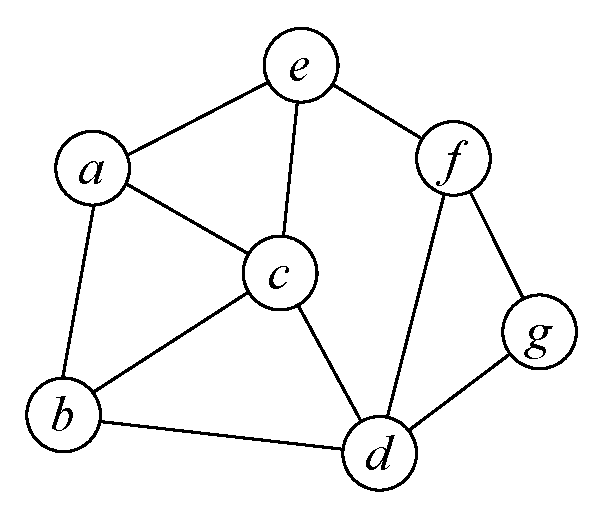
\includegraphics[scale=0.5]{figure/metis_inpg.eps}
\caption{Graph of partition target  \label{fig:mgpmetis_graph}}
\end{center}
\end{minipage}

\begin{minipage}{0.7\hsize}
\begin{center}
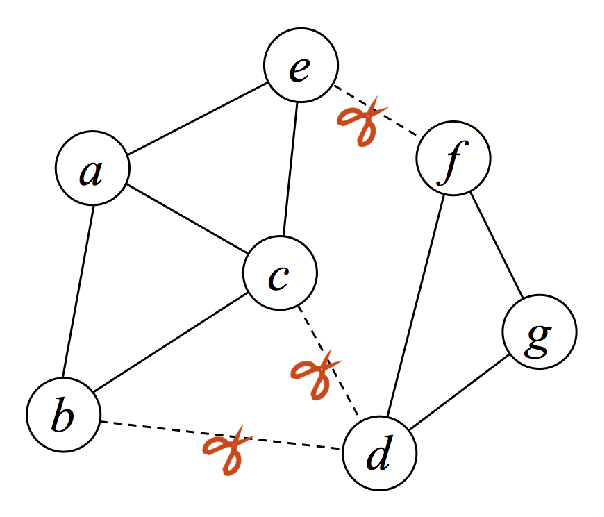
\includegraphics[scale=0.5]{figure/metis_gcut.eps}
\caption{Results of two partition after minimum cut. Since there are 7 nodes, partition closest to equal division is 4:3 partition, thus, this figure shows minimally, 3 edges are removed to create the partitions. \label{fig:mgpmetis_gcut}}
\end{center}
\end{minipage}

\end{tabular} 
\end{center}
\end{figure} 


\subsection{Format}
\begin{verbatim}
mgpmetis.rb kway= [ptype=rb|kway] ei= [ef=] [ew=] [ni=] [nf=] [nw=] [o=]
            [balance=] [ncuts=] [dat=] [map=] [-noexe] [--help]
\end{verbatim}

\begin{table}[htbp]
{\small
\begin{tabular}{ll}
\verb|ei=|    & : File name of branch (node pairs) [required]  \\
\verb|ef=|    & : Field name of node pair (two columns) in edge file [default: "node1,node2"]   \\
\verb|ew=|    & :Field name of weight in edge file [optional: weight is 1 when this is not specified]  \\
              & : Weight must be specified as an integer.   \\
\verb|ni=|    & : File name of node [optional]  \\
\verb|nf=|    & : Field name of node (1 column) in node file [default: "node"]  \\
\verb|nw=|    & : Field name of weight in node file (multiple fields can be specified) [optional:  weight is 1 when this is not specified]  \\
              & : Weight must be specified as an integer.  \\
\verb|o=|     & : Output file name [optional: default uses standard output ]  \\
\verb|kway=|  & : Number of divisions [required]  \\
\verb|ptype=| & : Partition algorithm [default: kway]   \\
\verb|balance=| & : Balanced partition parameter [default: when ptype=rb 1.001, when ptype=kway is 1.03 ]  \\
              & : Specify the $\beta$ value as shown in equation \ref{eq:gpmetis_problem2}. \\
%\verb|ufactor=| & : 分割アンバランスファクタ【デフォルト: ptype=rbの時は1、ptype=kwayの時は30】 \\
%                & : 式\ref{eq:gpmetis_problem2}における$(\alpha-1)*1000$の値を指定する。 \\
%                & : ex. $\alpha=1.5$に設定したければ、ufactor=500($(1.5-1)*1000$)と指定する。\\
\verb|ncuts=| & : The number of trials for initial value in partition phase [option: default=1] \\

\verb|dat=|   & : File name of the data used for METIS command.  \\
\verb|map=|   & : File name of the mapping data of node number corresponding to node name specified in i= parameter used for mgpmetis command.   \\
\verb|-noexe| & : Do not execute  METIS algorithm. This is used when only output data at dat=,map= parameters.  \\


%\verb|params| & : gpmetisに直接渡すパラメータ文字列を指定する。\\
%              & : ノーチェックで渡されるので、内容を理解して利用する。\\
%              & : 本コマンドで固定されているパラメータもあるため、指定できるパラメータについては注を参照のこと。\\
\verb|--help| & : Show help  \\

\end{tabular} 
}
\end{table} 

%\subsubsection{注}
%\verb|params=|で指定できるパラメータは以下の通り。詳細はアルゴリズムの節を参照のこと。
%\begin{table}[htbp]
%{\small
%\begin{tabular}{ll}
%\verb|-ptype=kway|  & 分割方法をk-分割法に切り替える。\\
%                    & 内部では再帰2分割法(-ptype=rb)に固定しているので、その方法を変更できる。\\
%                    & gpmetisコマンドのデフォルトは\verb|kway|であるが、本コマンドでは\verb|rb|としている。\\
%\verb|-iptype=|     & 再帰2分割法における、分割アルゴリズムを指定する。\\
%                    & \verb|nw=|を複数項目指定した場合\verb|grow|が、複数指定した場合は\verb|random|がデフォルトとなる。 \\
%                    & \verb|grow|: GGGP(Greedy Graph Growing Patitioning Algorithm) \\
%                    & \verb|random|: GGP(Graph Grawing Patitioning Algorithm) \\
%\end{tabular} 
%}
%\end{table} 


\subsection{Algorithm}
gpmetis is a graph partition algorithm that can be divided into three processes namely 1) coarsening, 2) partitioning 3) uncoarsening.
During coarsening, the process of integrating multiple nodes  connected by edges, and reduces to small graphs consisting of hundreds of nodes.   
In the coarsened graph, it is possible to obtain balanced partitions (with consideration of number of integrated nodes), while minimizing the number of cut on edges. 
Finally, the  uncoarsened process revert all partitioned nodes back to integrated nodes \ref{fig:mgpmetis_abst}.  

The features of gpmetis algorithm are as follows. 

It becomes difficult to solve a NP complete graph partitioning problem when the graph size increases. Therefore, gpmetis avoid the bottleneck by applying coarsening preprocessing technique to reduce the size of the graph. However, since coarsening reduces the flexibility of different ways to partition the graph,  the general partition accuracy (objective function that describes the minimisation of edge cut is described later) is decreased. 
Note that the algorithm in gpmetis is an approximation algorithm, thus optimal solution is not guaranteed. 


\begin{figure}[htbp]
\begin{center}
\begin{tabular}{cc}

\begin{minipage}{1.0\hsize}
\begin{center}
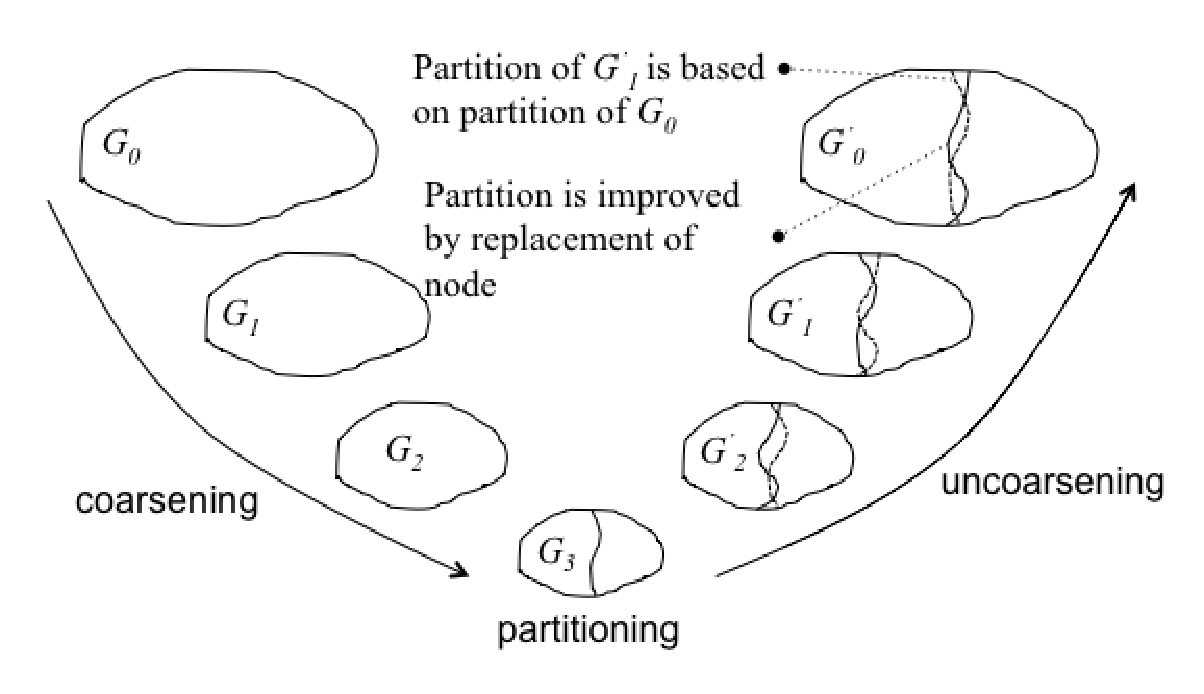
\includegraphics[scale=0.5]{figure/mgpmetis_abst.eps}
\caption{Conceptual diagram of multi-level graph partitioning (Refer to literature \cite{Karypis1999} of Figure 1).
In coarsening process, when the number of nodes reached several hundreds, original graph is reduced by merging the nodes to build condensed, smaller graphs. 
The reduced graphs have uniform number of nodes, with minimal number of edge cut for partition. In the uncoarsening process, the merged nodes are revert back to original. At that time, the nodes between partitions are replaced to improve the minimum cut. 
In the figure, $G_2$ and $G'_2$ consists the same node set, yet the cut edge set is different for partition purposes.} 
\label{fig:mgpmetis_abst}
\end{center}
\end{minipage}

\end{tabular} 
\end{center}
\end{figure} 



\subsubsection{Problem Setting}
In undirected graph  $G=(V,E)$, node set $V$ has $k$ number of partitions into $V_1,V_2,\dots,V_k$. 
In this case, the edges attached to partition is minimized (minimize edge cut), 
the nodes belong to each partition are divided equally. 
Generally, vertex $u,v$ extends edge to $(u,v)\in E$ with weight $w(u,v)\ge 0$, weight of node $v$ is represented as $w_v$, the function to minimize edge cut is represented in equation \ref{eq:gpmetis_problem1}. 
In addition, by introducing constraints to unify parameter $\beta\ge 1.0$ allows creation of uniform partitions (equation \ref{eq:gpmetis_problem2}). 
Balancing partitions corresponds to the ratio of average number of nodes (weight) in partition to the biggest number of nodes (weight), thus a larger  $\beta$ value allows for more unbalanced partition. 
$\beta$ can be specified by \verb|balance=| parameter in the command. 


%すなわち2つの目的関数をもつ問題として定式化する。
%より一般的に、頂点$u,v$に張られた枝$(u,v)\in E$の重みを$w(u,v)\ge 0$、
%節点$v$に与えられた重みを$w_v$で表すと、
%それぞれの目的関数は、式\ref{eq:gpmetis_problem1},\ref{eq:gpmetis_problem2}として定式化できる。
%また、一様の基準についてもより一般的に、節点$v$に与えられた重み$w_v$の合計を各パーティションで一様にすることを考える。
%ただし、一般に完全に一様にすることは難しいので、一様化パラメータ$\beta$を導入し、
%式\ref{eq:gpmetis_const}を満たす制約の元で式\ref{eq:gpmetis_problem}を最小化する。

{\footnotesize
\begin{equation}
\argmin_{V_1,V_2,\dots,V_k} \sum_{(u,v)\in E \wedge u\in V_i \wedge v\in V_j \wedge i\ne j} w(u,v) \\
\label{eq:gpmetis_problem1}
\end{equation}
}

{\footnotesize
\begin{equation}
\textrm{subject to}\ \ \frac{\max_i \sum_{v\in V_i} w_v}{\frac{1}{k} \sum_{i=1}^k \sum_{v\in V_i} w_v} \le \beta
\label{eq:gpmetis_problem2}
\end{equation}
}

%{\footnotesize
%\begin{equation}
%\argmin_{V_1,V_2,\dots,V_k} \frac{\max_i \sum_{v\in V_i} w_v}{\frac{1}{k} \sum_{i=1}^k \sum_{v\in V_i} w_v}
%\label{eq:gpmetis_problem2}
%\end{equation}
%}


%以上の多目的問題に対して、パレート解を列挙することも可能ではあるが、
%gpmetisでは、計算効率を優先させ、
%上記の2つの目的をできる限り達成するような分割を、以下で解説するアルゴリズムとして定義している。
%アルゴリズムの詳細についていは\cite{Karypis1999}を参照されたい。

%原著においては、特に以下の様な定式化は示されていない。
%目的関数のみならず、制約条件も満たさない近似解を出力することがある。
%グラフ分割問題にアルゴリズムにより定義したものと考える。

%以下、gpmetisの分割アルゴリズムを示すが、より詳細については\cite{}を参照されたい。

\subsubsection{Recursive bisection and k-way split}
gpmetis adopt an algorithm suitable for NP-complete graph partition problem, instead of finding the optimal solution, it is possible to apply multi-level partitioning, thereby making it possible to calculate increase in graph size at real  time. Multi-level partitioning generally follows several phases of the constructed algorithm.   
By contracting the original graph (referred to as coarsening), graph is divided when it is at a sufficiently small size. Afterwards,  when partition accuracy is improved (minimize edge cut), uncoarsening process will return the graph to original size. 

mgpmetis command comprised of two partition algorithm namely multi-level recursive bisection and multi-level k-way partition. 
When a node set  $V$ is divided into $k$ partitions, recursive bisection partition the original graph into two subgraphs through ``coarsening, partition, uncoarsening" phases, and recursively divides each of the partition
\footnote{
Recursive partition do not multiply $k$ by power of 2, weight of partitions are deliberately unbalanced so that it is possible to divide uniformly as a whole. For example, with $|V|=9, k=3$, it is initially partitioned into two parts at ratio of 3:6, afterwards, the 6 graphs are recursively partitioned into 3:3. The details are not shown in Algorithm\ref{algo:mgpmetis_1}. 
}.  

Recursively bisection is shown in Algorithm\ref{algo:mgpmetis_1}. 
 On the other hand, in k-way split method, the graph is directly partitioned into  $k$ parts after coarsening, and the process ends with uncoarsening. k-way partition is shown in  Algorithm\ref{algo:mgpmetis_2}. 
Either method provides excellent way of partition, in terms of execution time, k-way partition method is superior since it does not perform recursive partition\footnote{
Given $k=256$, it is reported that it is 3 to 4 times faster \cite{Karypis1998}.}.  
 

\begin{algorithm}
\caption{k split graph partition algorithm:\ \textbf{Recursive bisection}\label{algo:mgpmetis_1}}
\begin{small}
\begin{algorithmic}[1]
\Function{Bisect}{$G,P$}
	\State $G:Partition target graph, P: Partition set$
 	\If{size of $G$ is $1/k$}
		\State $P=P\cup \{G$\} 
	\Else
		\State $C$=Coarsen($G$) \Comment Coarsening
		\State $C_1,C_2$ = 2wayPartition($C$) \Comment Coarsen graph bisection 
		\State $G_1,G_2$ = Uncoarsen($C_1,C_2$) \Comment Uncoarsen
		\State $P$=\textsc{Bisect}($G_1,P$) \Comment $G_1$ in recursion 
		\State $P$=\textsc{Bisect}($G_2,P$) \Comment $G_2$ in recursion 
	\EndIf
	\State {\bf return}\ $P$
\EndFunction
\end{algorithmic}
\end{small}
\end{algorithm}

\begin{algorithm}
\caption{k split graph partition algorithm:\ \textbf{$k$-way partitioning method}\label{algo:mgpmetis_2}}
\begin{small}
\begin{algorithmic}[1]
\Function{Kway}{$G$}
	\State $G: Partition target graph$
	\State $C$=Coarsen($G$) \Comment Coarsening
	\State $C_1,C_2,\dots,C_k$ = KwayPartition($C$) \Comment Partition coarsened graph into k splits
	\State $G_1,G_2,\dots,G_k$ = UncoarsenKway(\{$C_1,C_2,\dots,C_k$\}) \Comment k split during uncoarsening
	\State {\bf return}\ \{$G_1,G_2,\dots,G_k$\}
\EndFunction
\end{algorithmic}
\end{small}
\end{algorithm}

In the following,  Algorithm\ref{algo:mgpmetis_1},\ref{algo:mgpmetis_2} shows each sample function, 
Coarsen(), 2WayPartition(), KwayPartition(), Uncoarsen(), UncoarsenKway() with summary below. 
Please refer to \cite{Karypis1999} for details. 

\subsubsection{Coarsen function)}
The purpose of coarsening is to reduce the size of the graph in order to perform partition efficiently. 
Coarsening algorithm is common to both recursive bisection and k-way partition. 
The coarsening phase finds out maximal matching $M$ from the original graph $G_0=(V_0,E_0)$, 
each element (edge) is merged with new node if matched, to create new graph $G_1=(V_1,E_1)$. 
Where graph $G=(V,E)$ matches $M$, and subset of edge set $E$ ($M \subseteq E$), the vertices of any 2 edges $e_1,e_2 \in M$ does not share the same edge set with each other. 
When matching $M$, if no more branches can be added, it is known as maximal matching. 
The above operation is applied recursively until the node size is at several hundred, a series of coarsened graphs $G_1,G_2,\dots,G_m$ are created. The details on finding maximal matching algorithm is not described in gpmetis. However, note that this method is based on a heuristic method using random numbers. 
 
\subsubsection{2WayPartition function, KwayPartition function)}
%粗化されたグラフを$k$個のパーティションに分割する方法として、再帰二分割法が用いられる。
%ここでも、マルチレベル再帰二分割法とマルチレベルk-way分割法で共通である。
%として、再帰二分割法(recursive bisection)とk-way分割法の2つの方法が利用できる。
%再帰2分割法では、2分割を再帰的に繰り返すことで、またk-way分割法では直接$k$個のパーティションに分割する。

%\paragraph{再帰二分割法}
%節点集合$V$を$k$個のパーティションに分割することを考えると、
%再帰二分割法では$\log_2 k$回の分割が必要となる。
%$k$が2のベキ乗でない場合は、単純にレベルの異なる分割を抑制することで対応する。
%例えば、$k=3$の場合、$V$を$V_1,V_2$に2分割した後、$V_1$は再帰的に二分割するが、$V_2$は分割を実施しない。
%このことによりアンバランスなパーティションができるが、逆粗化の過程におけるrefinement処理により調整される。


Below details 2 way partition for the coarsened graph $G=(V,E)$. 
Division of k number of partitions can be achieved by recursively applying bisection method. The bisection algorithm employed in gpmetis is very simple and emphases on efficiency. First, select the initial node randomly from the node set $V$, and connect with  another added node, the process ends when only half a node (total weight) is added. 
When the node is added to the node set, it is represented as  $P$,  there are two methods for $P$ to add node $v\in V\setminus P$, they are GGP(Graph Grawing Algorithm) andGGGP(Greedy Graph Growing Algorithm). 
GPP selects node $v$ randomly. Yet in GGGP,  $P$ is connected to $V\setminus P$ at which node $v$ has the greatest difference. Equation  $w(v,u)$ shows the edge extension weight between node $v$ and $u$. 
GGGP use greedy algorithm to reduce the number of cut when selecting node $v$. 
GGGP is applied in gpmetis by default, GGP is used when the weight constraints of node are specified more than once.

 
{\footnotesize
\begin{equation}
g_v=\sum_{(v,u)\in E \wedge u\in(P)} w(v,u)  - \sum_{(v,u)\in E \wedge u\in (V\setminus P)} w(v,u)
\label{eq:gpmetis_gggp}
\end{equation}
}


%GGP、GGGPのいずれの方法も、初期節点の選び方によって結果が変わってくる。
%そこで\verb|ncuts=|パラメータを指定することで、初期点を複数回選び、最も優れた分割を選ぶことができる。
%GGPとGGGPの使い分けは、パラメータ\verb|iptype=|によって指定する。

%またサイズのバランシングにおいて節点重みを複数指定した場合は、GGGPではなく、
%初期節点から隣接する節点を幅優先探索でランダムに選択する方法(GGP:Graph Grawing Algorithm)が用いられる。
%\end{description}

\subsubsection{Uncoarsen function, UncoarsenKway function)}
A series of coarsened graphs $G_1,G_2,\dots,G_m$ are obtained through the coarsen process. The reverse direction  ($G_m,G_{m-1},\dots$) returns the combined nodes and edges to the original state. Partition process  $G_m$ divides into $k$ partitions, if the partition is optimal, when  $G_m$ is returned to $G_{m-1}$, it may become less than optimal partitioning. Some of the nodes may be moved between partitions to improve partition accuracy (minimize edge cut). The above process is repeated until $G_0$ is obtained, which is the final solution of partition. 
 
 
\subsubsection{Other parameters}
The coarsening, partition, uncoarsening algorithm use random number, different result may be obtained by a series of random number. 
Therefore, when \verb|ncuts=| parameter is specified, the process of coarsening to uncoarsening is executed multiple times, thus it is possible to choose the best split. 
Recursive bisection method repeats the number of times specified in line 6,7,8 of Algorithm\ref{algo:mgpmetis_1}, and line 3, 4, 5 of Algorithm\ref{algo:mgpmetis_2}.   

In METIS, there are a number of parameters that can be used to control partitioning other than those from the mentioned above. 
This command can handle some of the parameters. If you want to set parameters that cannot be handled by this command, users can process data directly with METIS and create its processing data with this command. Specify the output data used by METIS at \verb|dat=| (node number is shown as integer in data). 


\subsection{Examples}
\subsubsection{Example 1. Example of the above illustration}
Partition into two parts using recursive bisection method(\verb|ptype=rb|). 
If the field name is not specified at \verb|ef=| in this command, field names of edge data is designated as  \verb|node1,node2| by default. 
 
\begin{Verbatim}[baselinestretch=0.7,frame=single]
$ more input.csv
node1,node2
a,b
a,c
a,e
b,c
b,d
c,d
c,e
d,f
d,g
e,f
f,g
$ mgpmetis.rb ei=input.csv o=output.csv kway=2 ptype=rb
$ more output.csv
node,cluster
a,1
b,1
c,1
d,0
e,1
f,0
g,0
\end{Verbatim}

\subsubsection{Example 2 . Specify node and edge weight}
Use of weight in column \verb|v| in \verb|edge.csv| file, and column  \verb|v| in 
\verb|node.csv| file. 
\begin{Verbatim}[baselinestretch=0.7,frame=single]
$ more edge.csv
n1,n2,v
a,b,1
a,c,1
a,e,1
b,c,1
b,e,1
b,g,2
c,d,3
c,g,1
d,e,1
e,f,1
$ more node.csv
n,v
a,1
b,1
c,3
d,1
e,1
f,1
g,3
$ mgpmetis.rb ni=node.csv ei=edge.csv o=rsl.csv ptype=rb kway=2 ef=n1,n2 nf=n nw=v ew=v
$ more rsl.csv
n,cluster
a,1
b,1
c,0
d,0
e,1
f,1
g,1
\end{Verbatim}

%\begin{thebibliography}{9}
%\bibitem{Bishop2008}
%C.M. ビショップ著, 元田浩, 栗田多喜夫, 樋口知之, 松本裕治, 村田昇(編), パターン認識と機械学習(下):ベイズ理論による統計的予測, 13章, pp.323--370, 2008.
%\end{thebibliography}

%\end{document}
%\end


